
\section{Counterexample} \label{sec:counterexample}

\begin{figure}[t]
	\centering
	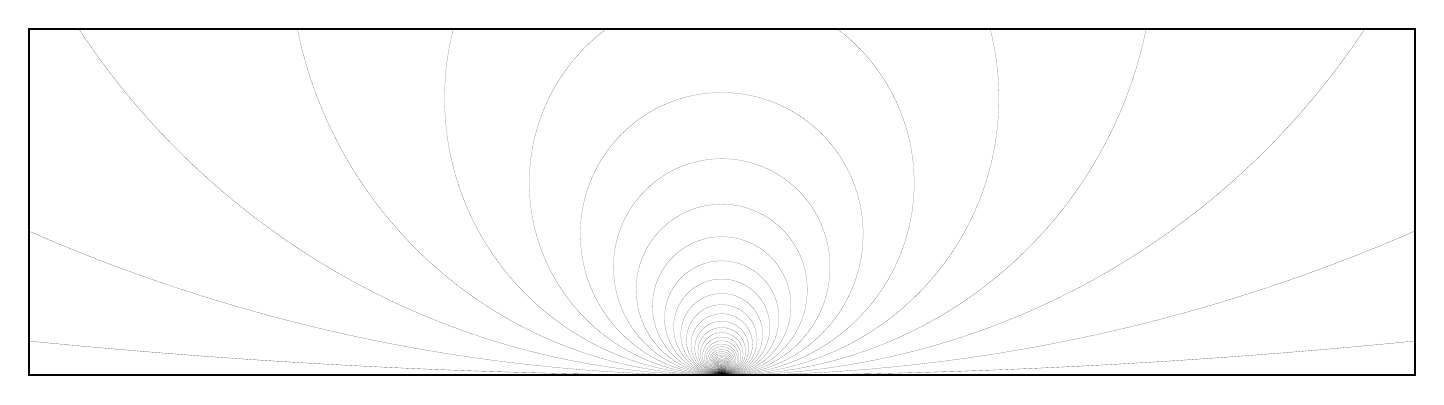
\begin{tikzpicture}[scale=88]
	\draw[thick] (-.1,0) rectangle (.1,.05);
	\clip (-.1,0) rectangle (.1,.05); % remove for all circles
	\foreach \i in {1,...,100}{
		\draw[line width=0.1/\i mm] (0, 1/\i^2) circle (1/\i^2);
	}
	\end{tikzpicture}
	\caption{TBW}
	\label{fig:earrings}
\end{figure}

In this section we show that a sublevel filtration can be $\HLC$ and not q-tame.

The $d$-dimensional Hawaiian earring is defined as the subspace
\begin{equation*}
\HE = \bigcup_{n\in\mathbb{N}}\left\{(x_0,\dots,x_d)\in\R^{d+1}\mid \left(x_0-\frac{1}{n}\right)^2+x_1^2+\dots+x_d^2=\left(\frac{1}{n}\right)^2\right\}
\end{equation*}
of $d+1$-dimensional Euclidean space.
Let $f \colon \HE\to\R$ as $0$ at the origin $\vec{0}$ and $1$ everywhere else.
All sublevel sets $\HE_{\leq t}$ are either the singleton $\{\vec{0}\}$ or the whole space $\HE$, and therefore compact.
Moreover, $\HE$ is locally-$f$-connected as we prove now. 

Let $e > 0$ and $p \in \HE$.
If $p$ is the origin, we choose $\delta$ between 0 and $\min\{e,1\}$.
Then $\HE_{\leq f(p) + \delta} = \HE_{\leq \delta} = \{p\}$, so the condition is trivially satisfied.
For $p$ not the origin, there is a unique $d$-sphere that contains it.
Clearly, we may choose $\delta$ so small that $B_{\delta}(p)$ contained in this sphere, so $B_{\delta}(p)$ is a disk and the condition follows trivially again. 

What remains to be shown is that $\HE_{\leq \bullet}$ is not q-tame with respect to singular and \v{C}ech homology.
Note that $\HE_{\leq t}$ is constant with value $\HE$ for $t \geq 1$, so it suffices to show that the singular and \v{C}ech homology of $\HE$ with field coefficients is infinite dimensional.
The case of singular homology is well know.
For \v{C}ech homology we use the fact that it commutes with inverse limits for compact Hausdorff spaces.
Define 
\begin{align*}
\HE_k &= \left\{(x_0,\dots,x_d)\in\R^{d+1}\mid \left(x_0-\frac{1}{k}\right)^2+x_1^2+\dots+x_d^2=\left(\frac{1}{k}\right)^2\right\}\\
&\cup\bigcup_{n=1}^{k-1}\left\{(x_0,\dots,x_d)\in\R^{d+1}\mid \left(x_0-\frac{1}{n}\right)^2+x_1^2+\dots+x_d^2=\left(\frac{1}{n}\right)^2\right\},
\end{align*}
i.e., the $d$-dimensional Hawaiian earring but with the $k$-th largest $d$-sphere filled.
We have $\lim_{k}\HE_{k} = \bigcap_{k}\mathbb{H}^{d}_{k}=\mathbb{H}^{d}$, and hence $\CH_{d}(\HE) = \lim_{k}\CH_{d}(\mathbb{H}^{d}_{k})$.
One can easily check that each $\mathbb{H}^{d}_{k}$ satisfies the assumptions for \cref{prop:cech_sing_hom_hlc}, which implies $\lim_{k}\CH_{d}(\mathbb{H}^{d}_{k})=\lim_{k}H_{d}(\mathbb{H}^{d}_{k})$.
We compute
\[
\lim_{k}H_{d}(\mathbb{H}^{d}_{k})=\lim\left(\dots\to \prod_{n=1}^2\mathbb{F}\to \prod_{n=1}^1\mathbb{F}\to \prod_{n=1}^0\mathbb{F}\right)=\prod_{n\in\mathbb{N}}\mathbb{F},
\]
which is infinite-dimensional over $\mathbb{F}$.
This finishes the proof.

\begin{rem}
Note that the singular persistent homology of the sublevel set filtration of $F$ above is also not q-tame because the $d$-dimensional Hawaiian earring has infinite-dimensional $d$-th singular homology \cite{Barratt.1962}. 
\end{rem}

\begin{rem}
The construction above does not yield a counterexample to \cref{con:q-tame_pers_cech_hom} because $\mathbb{H}^{d}$ is not strongly locally-$F$-connected at the origin.
\end{rem}